\documentclass[12pt, a4paper,oneside]{article}

\usepackage{multirow}
\usepackage{graphicx}
\graphicspath{ {references/} }


\usepackage{float}%figures placed HERE

\usepackage[backend=bibtex]{biblatex}
\bibliography{miniproject}
%\bibliographystyle{plain}


\title{Reconfigurable and Low Energy Systems Miniproject\\\large CORDIC}
\author{Anders Normann Poulsen (apouls16@student.aau.dk)\\Gabriel Vasluianu (gvaslu16@student.aau.dk)}


\begin{document}

\maketitle
\newpage
\section{Introduction}
CORDIC is an algorithm that computes trigonometric functions (and many other)
by using simple operations.
%https://en.wikipedia.org/wiki/CORDIC
A typical application would be a two-dimensional vector rotation, as seen in 
figure \ref{fig:two_vector}. Here $(x_{in}, y_{in})$ are the initial coordinates
of the vector, and $(x_{out}, y_{out})$ are the final coordinates.

\begin{figure}[h]
	\centering
	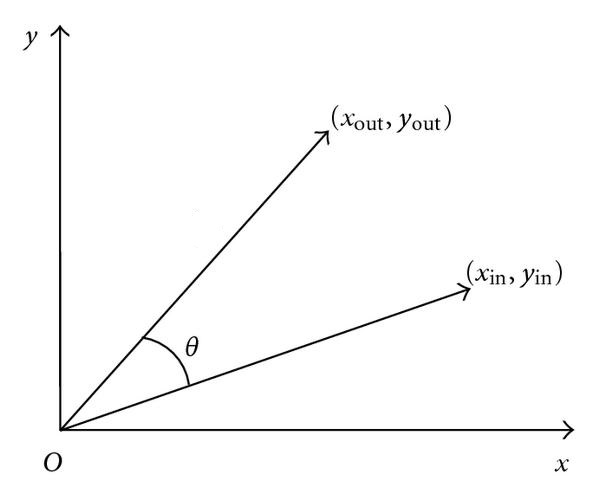
\includegraphics[width = 7cm]{two_vector.jpg}
	\caption{Two dimensional vector rotation}
	\label{fig:two_vector}
\end{figure}

In order to achieve the operation of rotating the vector, the following equations
have to be calculated:
\[ x_{out} = x_{in} cos\theta - y_{in} sin\theta \]
\[ y_{out} = x_{in} sin\theta + y_{in} cos\theta \]

As seen here, the hardware computing these equations would have to do:
four multiplications, two addition/subtraction 
and access a lookup table for the trigonometric functions\cite{cordic1}.
Keep in mind that multiplication is an expensive operation, and a multiplicator
takes a large area. This is the reason why we want to use CORDIC in some 
applications.
\\

The idea CORDIC introduces is that we can compute the new coordinates by 
iterating through an algorithm that constantly tries to get closer to the 
final result, using a table containing angles to be used in the next iteration
(micro-rotation). These angles can be either added or subtracted in order
to take the next step, and approximate the target, as seen in figure \ref{fig:cordic_iterations}.

\begin{figure}[H]
	\centering
	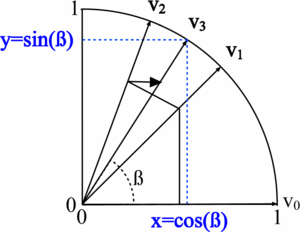
\includegraphics[width = 7cm]{cordic_iterations.png}
	\caption{Ilustration of cordic iterations. V3 is the desired rotation for V0,
	while V1 and V2 are the approximation steps CORDIC takes\cite{cordic2}}
	\label{fig:cordic_iterations}
\end{figure}

The generalized equations of the CORDIC algorithm are:
\[ x_{i+1} = x_i - \sigma_i \cdot 2^{-i} \cdot y_i \]
\[ y_{i+1} = \sigma_i \cdot 2^{-i} \cdot x_i + y_i\]
\[ z_{i+1} = z_i - \sigma_i \cdot arctan(2^{-i}) \]

%https://en.wikibooks.org/wiki/Trigonometry/For_Enthusiasts/The_CORDIC_Algorithm

Here, $x_{i+1}$ and $y_{i+1}$ show us the values respective to each iteration.
In order to know what to do in the next iteration (add/subtract from the previous
angle), we need to compute $\sigma_i$. This is done by looking at the value of 
$z_i$:

$$
\sigma_i = \left\{ \begin{array}{rl}
 +1 &\mbox{ if $z_i>=0$} \\
 -1 &\mbox{ if $z_i<0$}
       \end{array} \right.
$$

$z_i$ keeps track of how much we rotated at every iteration and subtracting that 
from the wanted angle.
The values of $x_i$ and $y_i$ need to be scaled by a factor of $K_i$:

$$K_i = \frac{1}{\sqrt{1 + 2^{-2i}}}$$

However, there are several methods to do this by calculating it in advance or by 
making it a constant. For small architectures, this aspect can be disregarded.
\\
This being said, by looking at the equations we can see that we will need 
to apply the following operations: addition and bitshift.

\section{From algorithm to architecture}

\subsection{Data flow graph (DFG)}
The data flow graph in figure \ref{fig:cordic_dfg} presents the data dependencies
in the CORDIC algorithm. There are two bit shifting operations, and three
addition/subtraction operations. 

%More information about how these operations
%are executed can be found in \ref{ssec:cdfg}. 

The group had difficulties 
in completely understanding how the interdependency between $x_{i+1}$
and $y_{i+1}$ will affect the architecture of the system.

\begin{figure}[H]
	\centering
    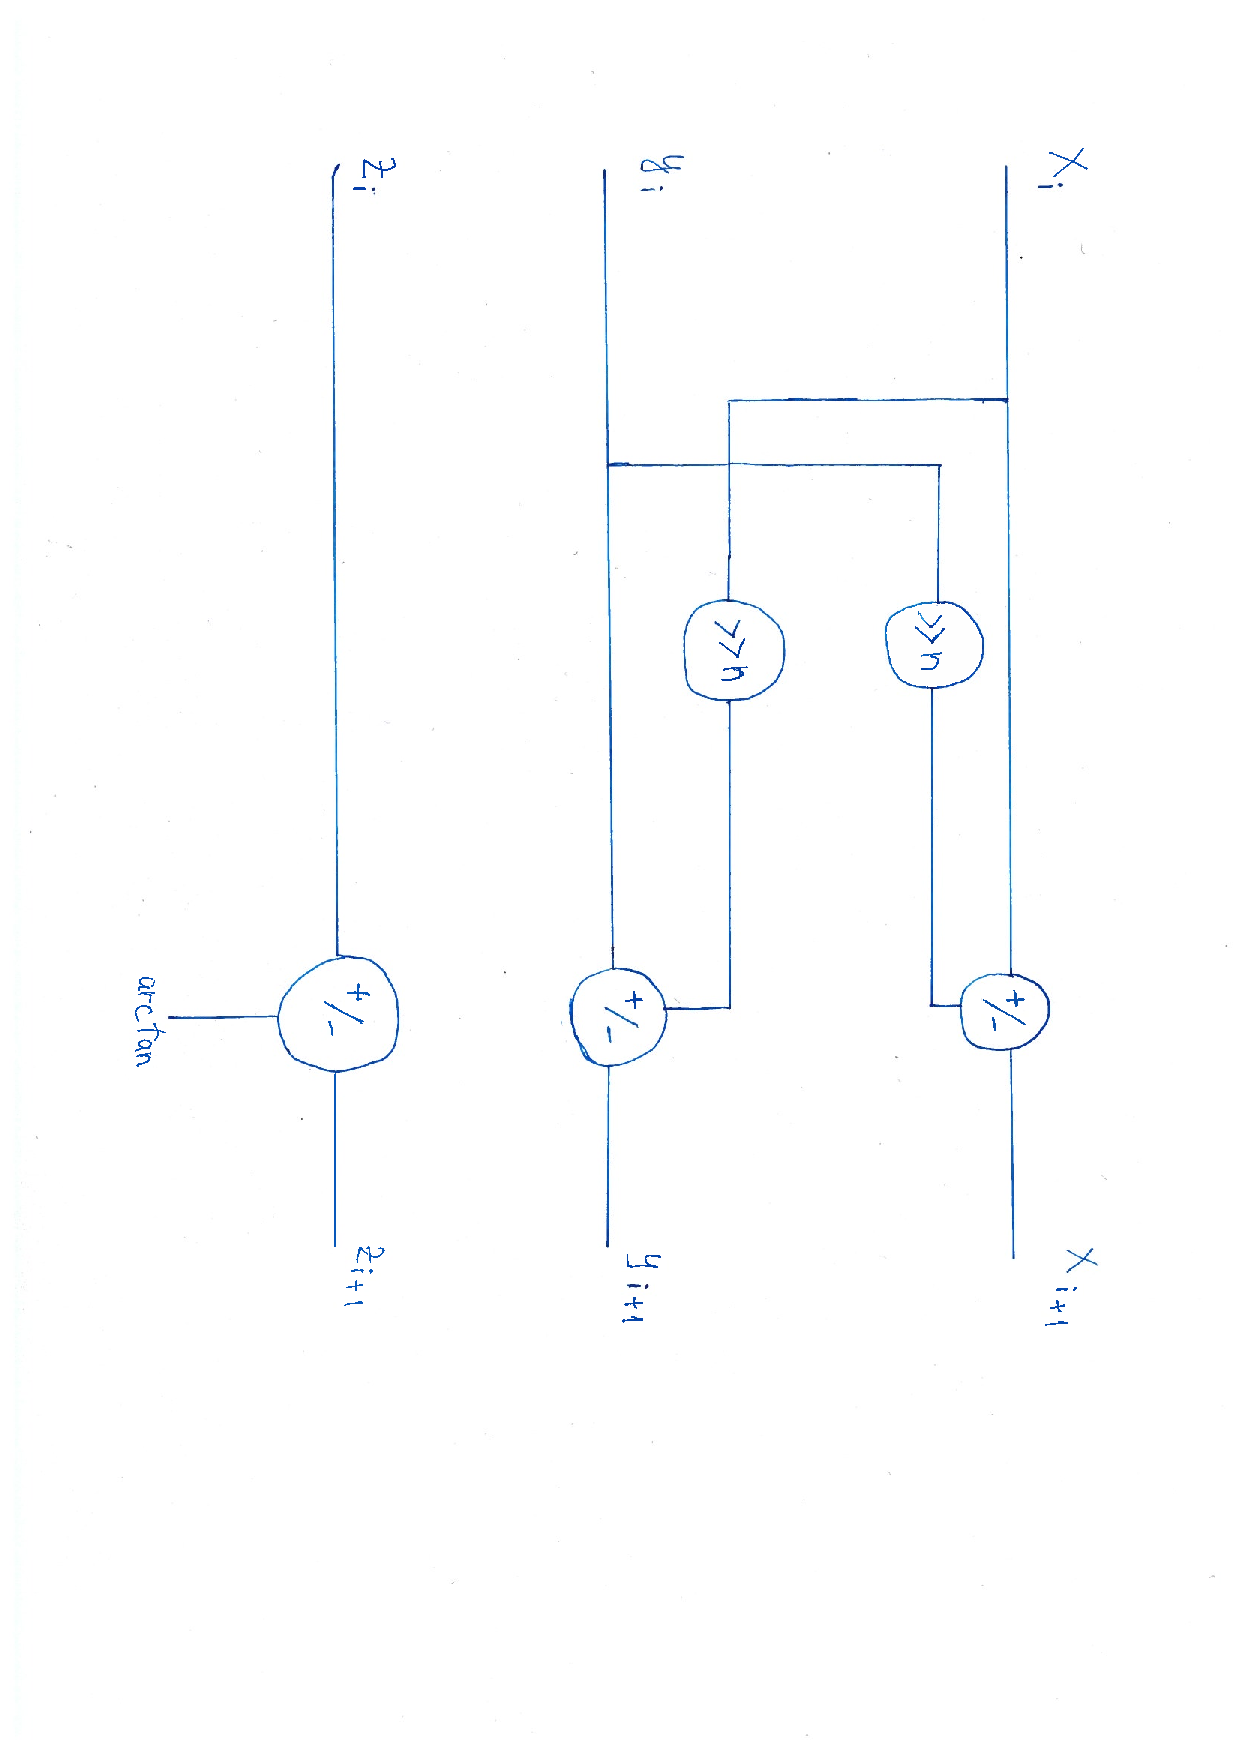
\includegraphics[clip, trim=2cm 7cm 2.2cm 2.5cm, width = 10cm,angle=90]{cordic_dfg.pdf}
	\caption{Data flow graph for CORDIC}
	\label{fig:cordic_dfg}
\end{figure}

The two shift operations ($>>n$) represent the $2^{-i}$ part of each transfer 
function. This has to be controlled by $i$. The same applies for the to 
additions, for computing $x_{i+1}$ and $y_{i+1}$, which will in fact 
either add or subtract the result of the shift, based on $z_i$. These aspects
will be analysed in \ref{ssec:fsdm}. $z_i$ relies on a table containing the 
values of precomputed values for $arctan$. This is stored in ROM, and will
contain the as many values, as the number of iterations the CORDIC algorithm 
is designed to take.

\subsection{Precedence graph (PG)}
The precedence graph in figure \ref{fig:cordic_pg} shows the ordering of the operations
from the DFG. This reveals the fact that the three computations, $x_{i+1}$; $y_{i+1}$ and $z_{i+1}$, can be executed 
in parallel if the necessary functional units are present.

\begin{figure}[H]
	\centering
	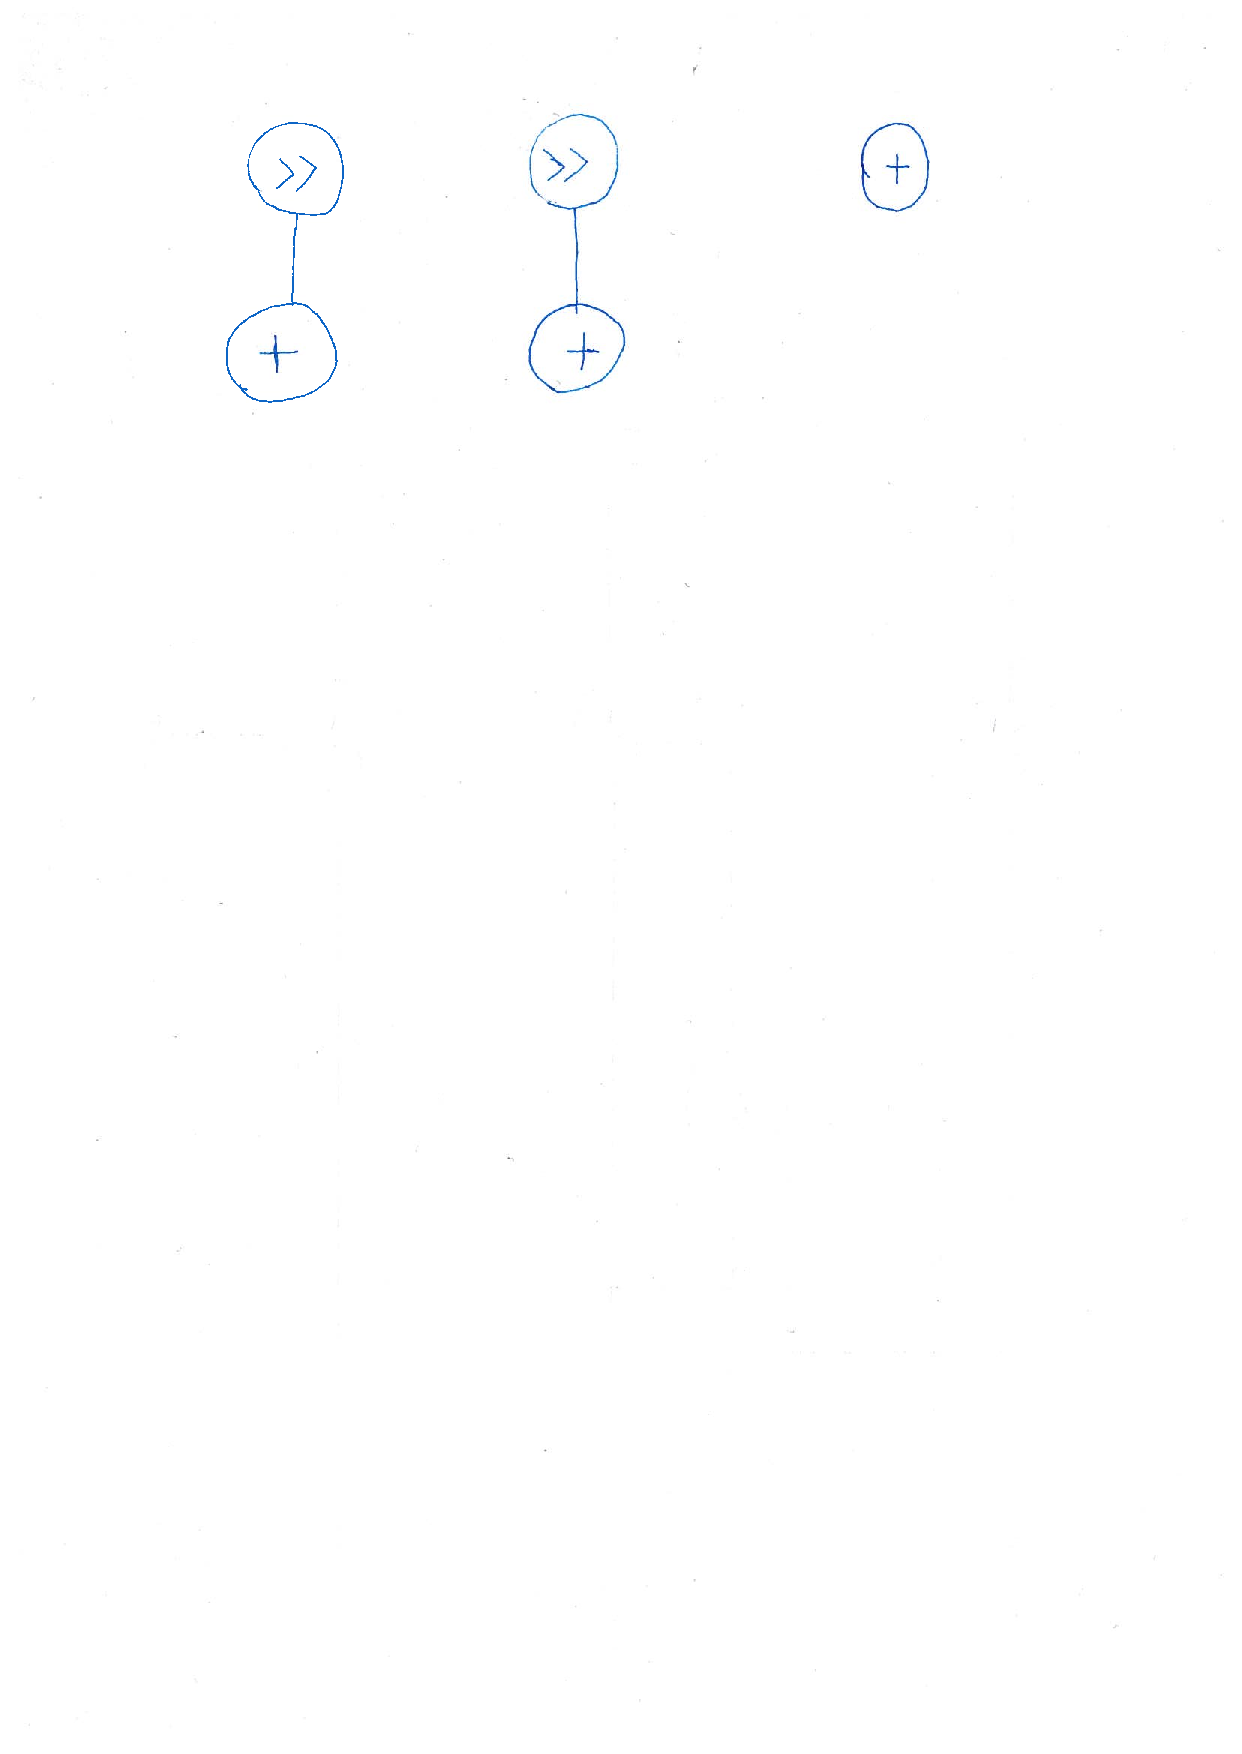
\includegraphics[width = \linewidth,trim=0 22.9cm 0 2cm, clip]{sequencediagram.pdf}
	\caption{Precedence graph for CORDIC}
	\label{fig:cordic_pg}
\end{figure}

Based on the precedence graph, we can now look into the hardware necessary for
computing the CORDIC algorithm. At this point, there is no reason to further
analyse the precedence graph. This is only composed of two identical 
critical paths (shift and addition) and an addition.

\subsection{Hardware mapping} \label{hw_mapping}
Figure \ref{fig:schedules} represents two ways of mapping the operations in the
CORDIC algorithm to functional unit. On the right side of the drawing, each operation
is executed on its own shifter/adder. The characteristics of this setup are:

\begin{itemize}
	\item 2 shifters
	\item 2 adders
	\item execution time is 2 time units
	\item the area for building the hardware is presumably large, but the execution time
	is short
\end{itemize}


On the left side of figure \ref{fig:schedules}, an ALU is shared for all the
operations:

\begin{itemize}
	\item 1 ALU able to execute addition, subtraction and bit shifting
	\item execution time is 5 time units
	\item the area occupied by the ALU is small, but the execution time is long.
	We should also keep in mind that we need to add some delays in the DFG so
	that the data is available at the proper time for the ALU to compute.
	These delays materialise in registers, which will increase the area slightly.
\end{itemize}

\begin{figure}[h]
	\centering
	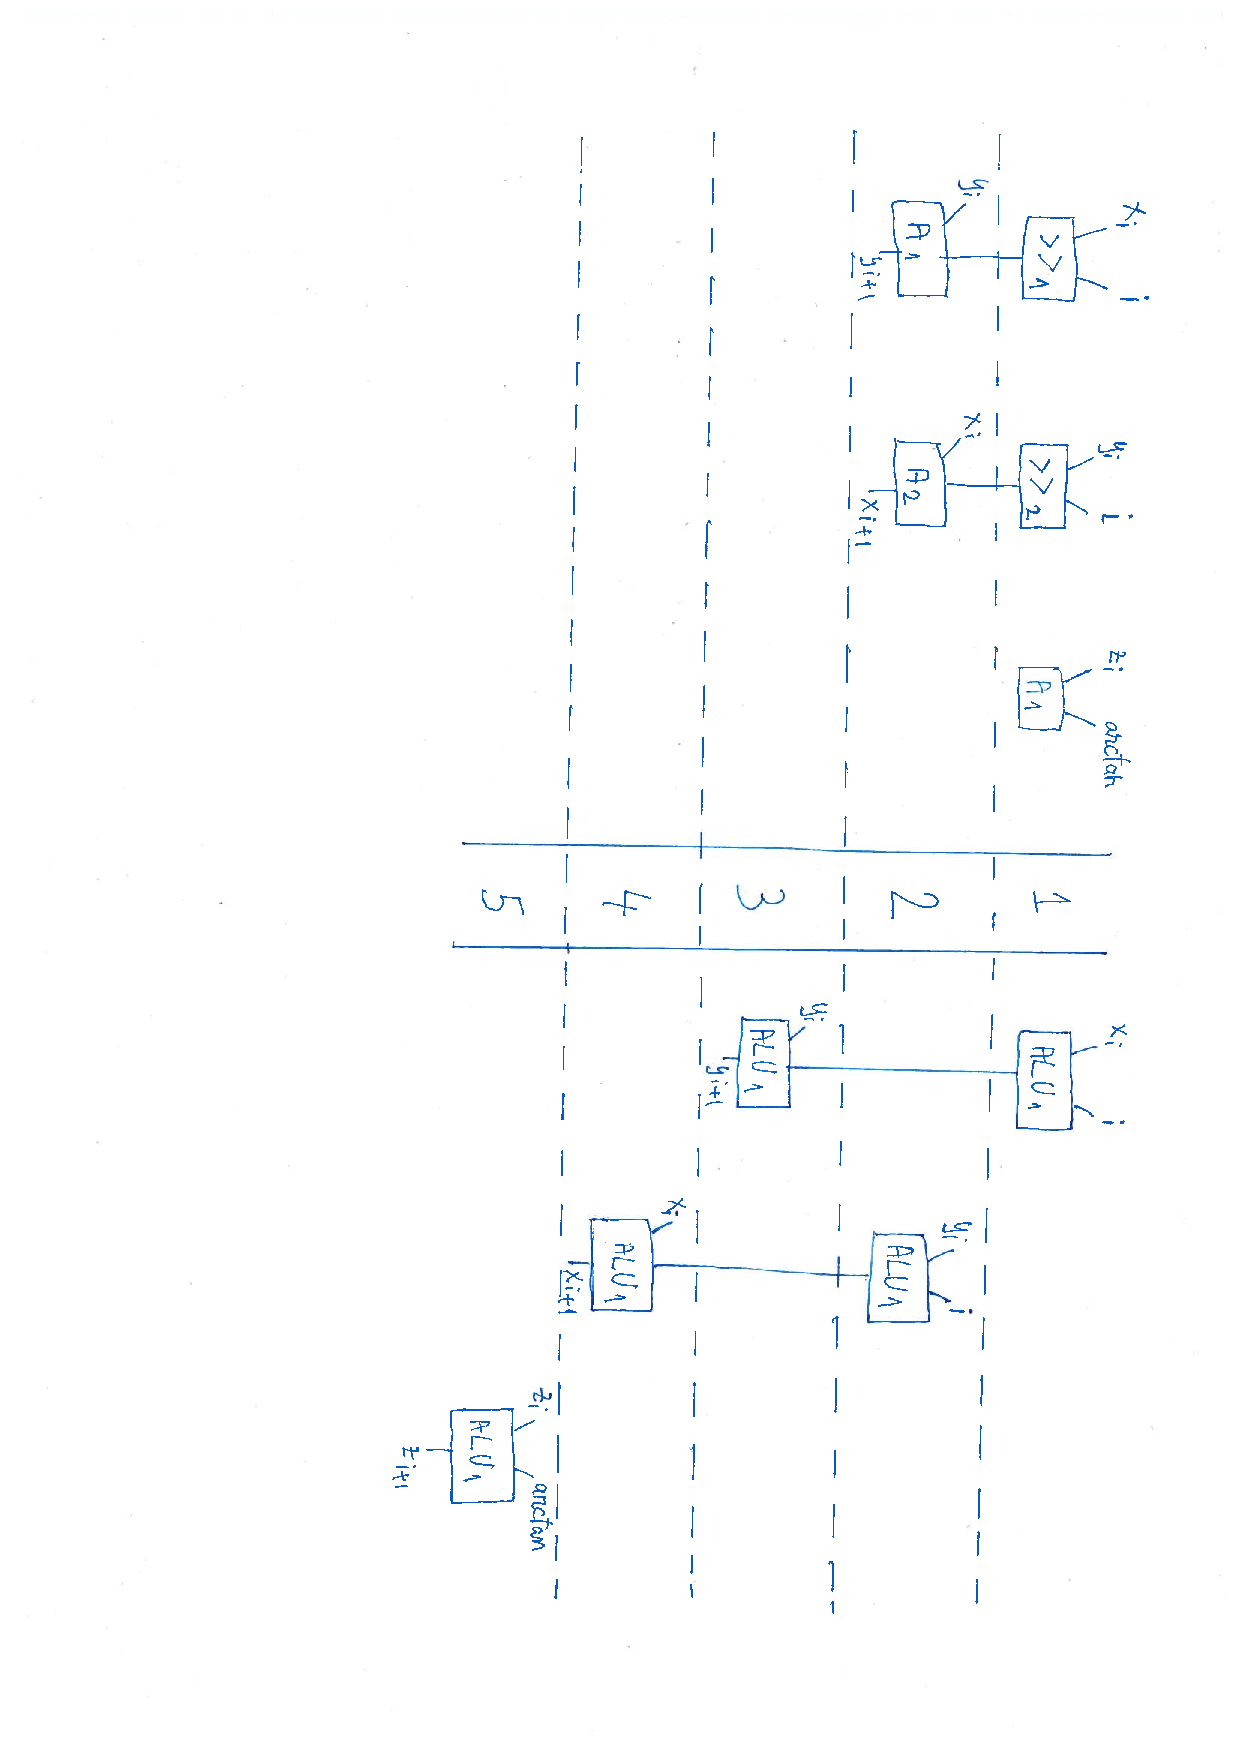
\includegraphics[height = \textwidth,angle=91, trim=6.5cm 3.5cm 1.5cm 3cm, clip]{schedules.pdf}
	\caption{1:1 hardware mapping, and fully shared ALU for CORDIC}
	\label{fig:schedules}
\end{figure}

Figure \ref{fig:schedules_1} represents some intermediate solutions to mapping
the hardware. In the first scenario, on the right side there is:

\begin{itemize}
	\item 1 shifter
	\item 1 ALU
	\item execution time is 3 time units
	\item This solution includes a physical shifter, instead of using the
	ALU. The shifter has such a simple functionality, that it should not too
	much to the area. However, by doing this, the execution time is reduced by 2
	time units, in comparison to the purely ALU solution
\end{itemize}

\begin{figure}[H]
	\centering
	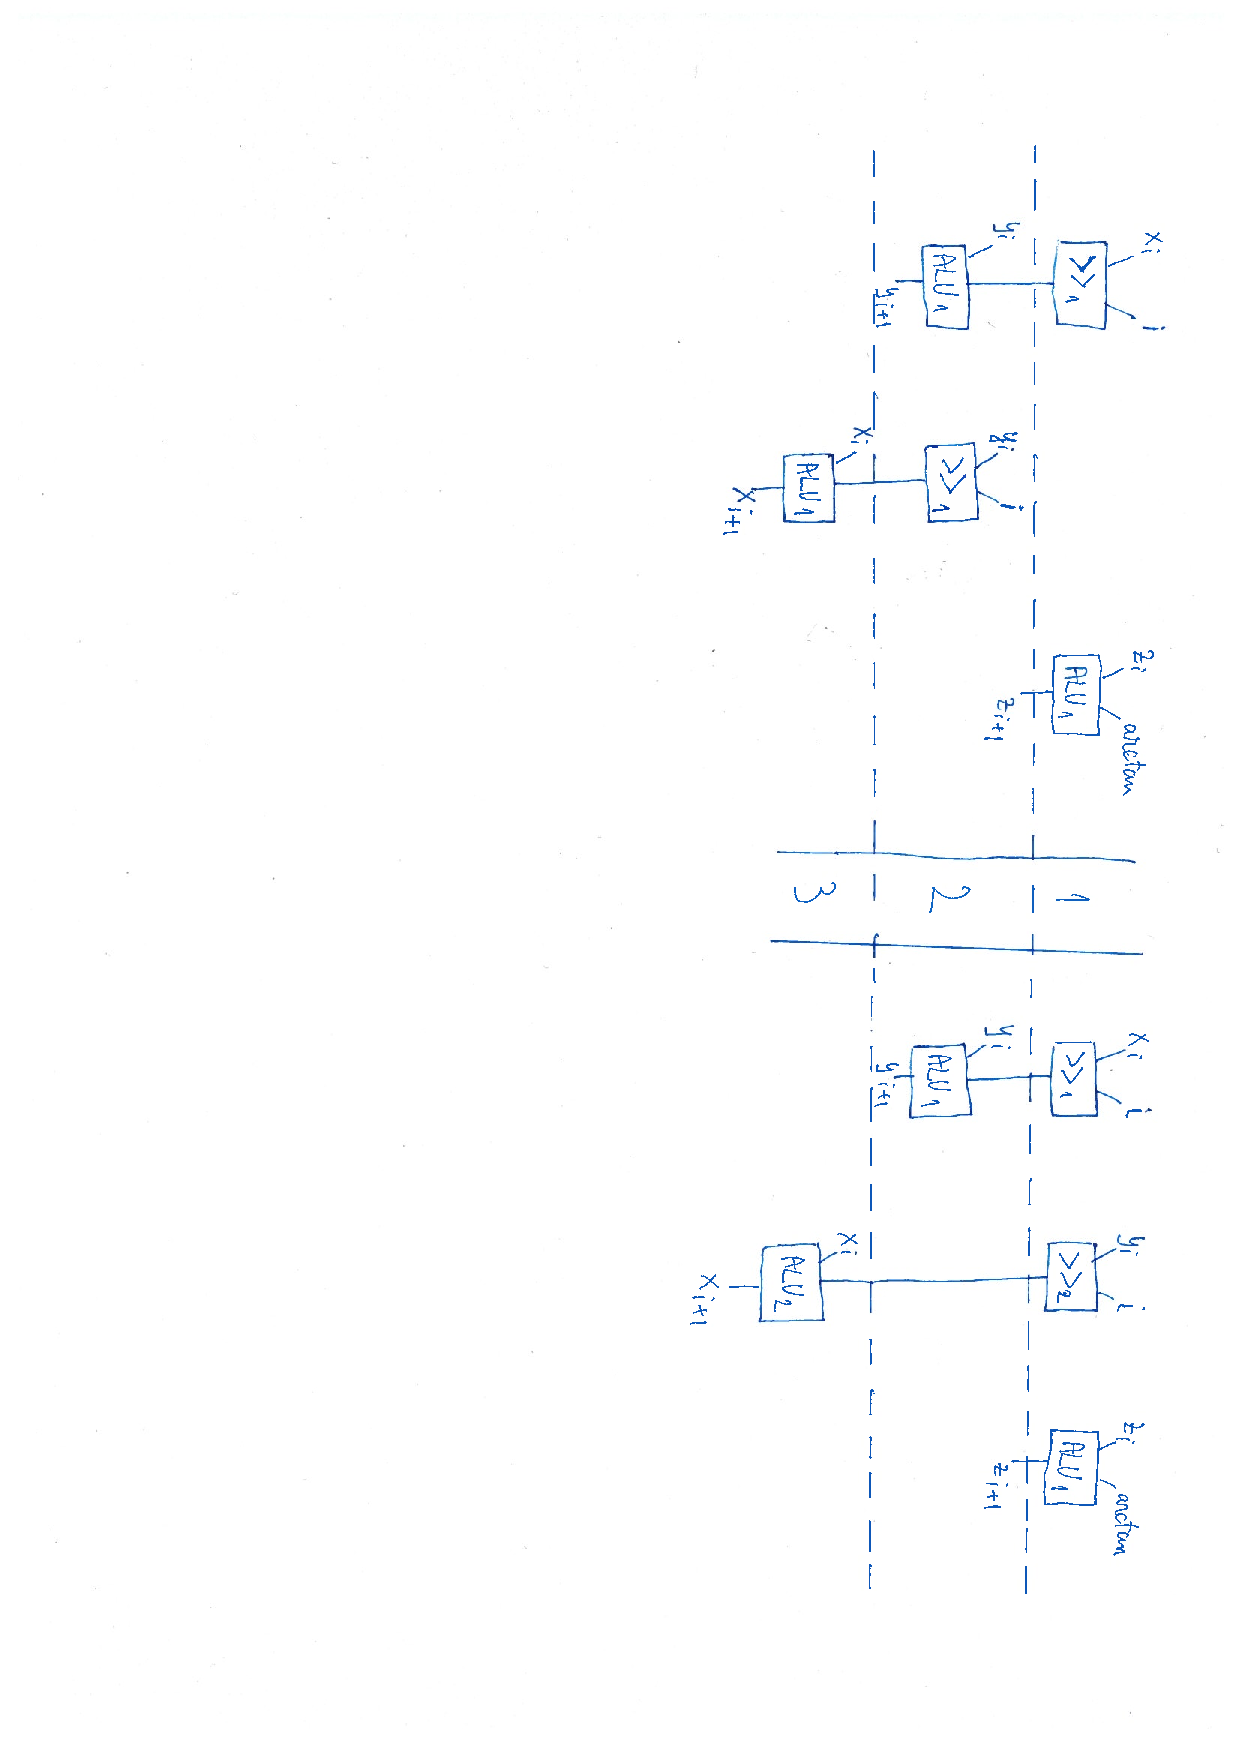
\includegraphics[height = \textwidth,angle=91, trim=11.5cm 3.5cm 1.5cm 3.5cm, clip]{schedules_1.pdf}
	\caption{Middle ground for hardware mapping for CORDIC}
	\label{fig:schedules_1}
\end{figure}

On the left side of the drawing there is yet another variation of the architecture:

\begin{itemize}
	\item 2 shifters
	\item 1 ALU
	\item execution time is 3 time units
	\item Here can be seen that by using two separate shifters, the execution time
	is not improved. There might be other algorithms where this approach might have worked,
	but this is not the case of CORDIC.
\end{itemize}

As seen in the figures, the group mainly focused on the \textit{Bit parallel,
iterative} implementation. This means that the algorithm will be iterated on 
the same hardware for a number of times, before outputting the final result.
Typically, 40 iterations are enough for most purposes, as the result will be \
correct to the 10th decimal place\cite{cordic2}. What this means in practice,
is that $i$ will be counting up to 40, and the $arctan$ table stored in ROM
will have the values for the first 40 angles.

\subsection{Finite state machine with data path (FSDM)}\label{ssec:fsdm}
A finite state machine dictates the states a system has to go through.
For our CORDIC algorithm, we have to start it, keep track of the iterations
and stop it when we are done computing with the desired accuracy. 
The data path represents the data processing operations taken by the hardware.
Figure \ref{fig:finite_state_machine} represents the FSDM for our CORDIC
implementation. The red box is the finite state machine, containing 5 states,
red lines are the control path and blue units denote the data path.

\begin{figure}[H]
	\centering
	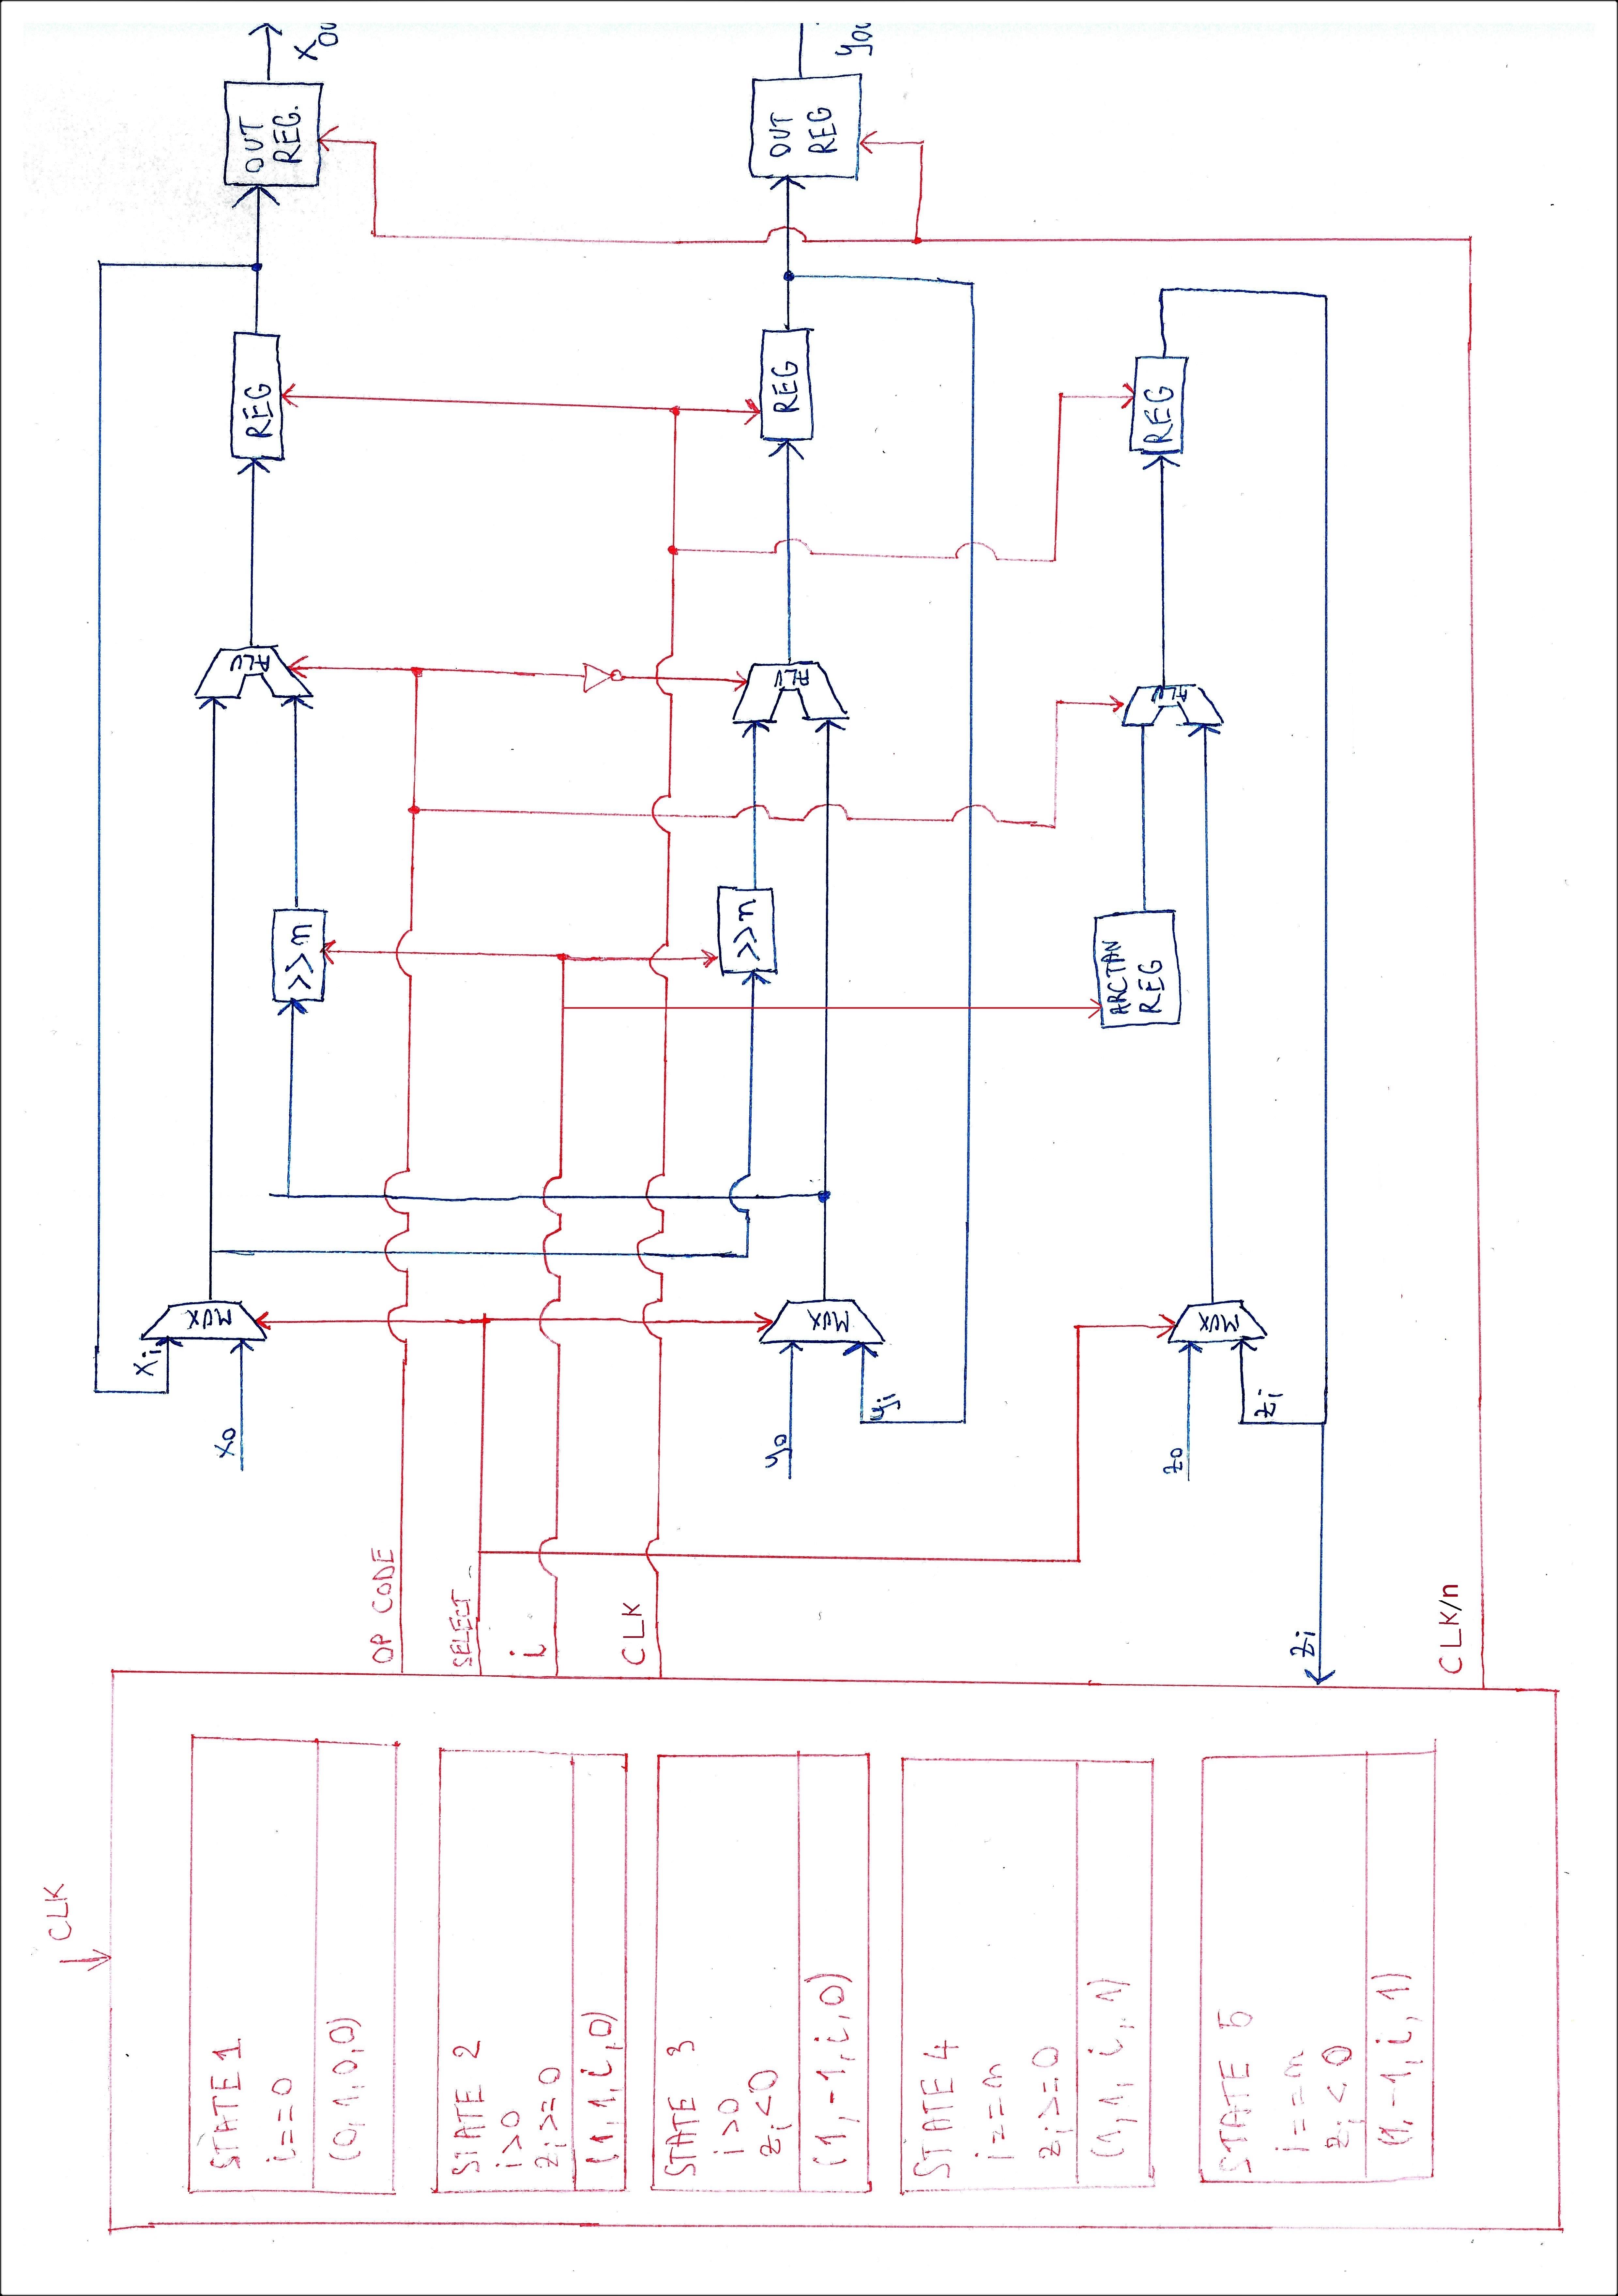
\includegraphics[width = \linewidth]{finite_state_machine_edit.jpg}
	\caption{Finite State Machine with Data Path}
	\label{fig:finite_state_machine}
\end{figure}

\paragraph{The data path}
contains the functional units discussed in \ref{hw_mapping}, in the 1:1 mapping
scenario. The inputs are the initial values of $x_0$, $y_0$ and $z_0$. The outputs
$x_{out}$ and $y_{out}$
come out of the output register, after the algorithm has executed the desired
number of times. All the functional units are controlled by the control unit, 
through the red control paths. $z_i$ is fed back into the control unit, 
so that it can decide the sign to be used in the next iteration.

\paragraph{The controller}
contains the states the system has to go through. The control unit takes
$z_i$ as input. Based of the value of $z_i$ and $i$ it computes the next state.
$i$ is not modelled in the figure; it works by incrementing its previous
value by 1. Each state is characterised by its outputs, on the control
path. These are:

\begin{itemize}
	\item select - telling the multiplexers whether to choose the initial 
	inputs  $x_0$, $y_0$ and $z_0$, or use the previous values of 
	$x$, $y$ and $z$
	\item OP code - telling the ALUs the operation they need to execute:
	addition and subtraction. Note that it is assumed that the ALU is simple and can only
	compute additions and subtractions. Thus, OP code can be binary, and for the computation
	of $y_{i+1}$ the OP code can simple be inverted to reflect the CORDIC algorithm precisely
	\item i - the current iteration. This is used by the shifters, to 
	know the number of positions they need to shift, and by the $arctan$
	lookup table
	\item CLK - the clock signal telling the registers when to release their
	values, in order to start the next iteration. CLK/n is the clock scaled
	to pulse only on every $n^{th}$ pulse. It is used to instruct the output registers
	when to output the final values of the computations
\end{itemize}

These control outputs can be seen at the bottom of each state, the notation for them being:
\[(select,\, OP\, code,\, value\, of\, i,\, CLK/n\,(output\, the\, values))\]
Where $n$ denotes the number of iterations.

These are the five states:
\begin{table}[H]
	\centering
	\begin{tabular}{| c | c c c c c |}
	\hline
		\multirow{2}{*}{Conditions}
				& $i = 0$			& $i > 0$ 			& $i > 0$			& $i = n$			& $i = n$		\\
				& 					& $z_i >= 0$ 		& $z_i < 0$			& $z_i >= 0$		& $z_i < 0$		\\
	\hline
		State	& $(0, 1, 0, 0)$	& $(1, 1, i, 0)$	& $(1, -1, i, 0)$	& $(1, 1, i, 1)$	& $(1, -1, i, 1)$						\\
	\hline
	\end{tabular}
\end{table}

\newpage
\printbibliography

\end{document}